\documentclass[10pt]{article}
\usepackage[a4paper,margin=18mm]{geometry}
\usepackage{amsmath,amssymb,booktabs,array,enumitem}
\usepackage[T1]{fontenc}\usepackage{lmodern}
\usepackage{tikz}\usetikzlibrary{shapes.gates.logic.US,positioning,arrows.meta,patterns,calc}
\usepackage[hidelinks]{hyperref}
\setlength{\parindent}{0pt}\setlength{\parskip}{4pt}
\setlength{\emergencystretch}{2em}
\newcommand{\VDD}{V_{DD}}
\newcommand{\mos}[4]{\begin{scope}[shift={(#1,#2)}]
\draw (0,.24)--(0,-.24);\draw (0,.20)--(.25,.20)--(.25,.5);
\draw (0,-.20)--(.25,-.20)--(.25,-.5);\draw (-.16,.23)--(-.16,-.23);
\ifnum#4=1\draw (-.26,0) circle (.06);\draw (-.75,0)--(-.32,0);\else\draw (-.75,0)--(-.16,0);\fi
\node[anchor=east,font=\scriptsize] at (-.76,0) {$#3$};\end{scope}}
\newcommand{\ground}[2]{\draw (#1,#2)--(#1,{#2-.12});\draw ({#1-.17},{#2-.12})--({#1+.17},{#2-.12});\draw ({#1-.11},{#2-.20})--({#1+.11},{#2-.20});}
\newcommand{\rail}[3]{\draw (#1,#2)--(#1,{#2+.14});\node[above,font=\scriptsize] at (#1,{#2+.14}) {$#3$};}

\newcommand{\hmos}[4]{\begin{scope}[shift={(#1,#2)}]
\draw(-.24,0)--(.24,0);\draw(-.2,0)--(-.2,-.25)--(-.5,-.25);\draw(.2,0)--(.2,-.25)--(.5,-.25);
\draw(-.23,.16)--(.23,.16);
\ifnum#4=1\draw(0,.26)circle(.06);\draw(0,.32)--(0,.75);\else\draw(0,.16)--(0,.75);\fi
\node[below,font=\scriptsize]at(0,-.32){#3};\end{scope}}
\newcommand{\gnd}[2]{\ground{#1}{#2}}\begin{document}
\begin{center}{\Large\bfseries 2021 Final -- Corrected Partial Solutions}\\EE3032 Introduction to VLSI Design, NCU\end{center}
This packet answers intact readable Q1--Q5 and Q7(a)--(c). It preserves Q6's readable fragments and diagram, but skips all numerical/pipeline answers because the original parameters and Q6(a),(b) are missing. Q7(d)--(f) is a separately labeled unverified typed supplement, with conditional conceptual notes. Original photographs govern circuit polarity, contacts, and assumptions; the corrected student set and later typed notes are comparison evidence.

\textbf{1. Cascaded domino logic (15 points)}
\textbf{(a)} Use an NMOS evaluation chain $A$--$B$ and a clocked footer, a PMOS precharge device, and a restoring inverter for the AND output $U$. The second domino gate has parallel NMOS inputs $U,C$, its footer/precharge pair, and an output inverter. Thus $U=AB$ and $Y=U+C$ during evaluation.
\begin{center}\begin{tikzpicture}[scale=.69,font=\scriptsize]
\mos{2}{5}{\phi}{1}\rail{2.25}{5.5}{V_{DD}}\mos{2}{4}{A}{0}\mos{2}{3}{B}{0}\mos{2}{2}{\phi}{0}\ground{2.25}{1.5}
\draw(2.25,4.5)--(3.7,4.5)--(3.7,3.5)--(4.25,3.5);\draw(3.7,3.5)--(3.7,2.5)--(4.25,2.5);\mos{5}{3.5}{\phantom{z_A}}{1}\mos{5}{2.5}{\phantom{z_A}}{0}\rail{5.25}{4}{V_{DD}}\ground{5.25}{2}
\draw(5.25,3)--(6.0,3)node[above]{$U=AB$};\node[left]at(2.25,4.5){$z_A$};
\mos{10}{5}{\phi}{1}\rail{10.25}{5.5}{V_{DD}}\mos{9}{3.5}{\phantom{U}}{0}\mos{11}{3.5}{C}{0}\draw(9.25,4)--(9.25,4.5)--(11.25,4.5)--(11.25,4);\draw(10.25,4.5)--(10.25,4.5);\draw(9.25,3)--(11.25,3);\mos{10}{2.5}{\phi}{0}\ground{10.25}{2}
\draw(6,3)--(7.5,3)--(7.5,3.5)--(8.25,3.5);\node[above]at(10.25,4.5){$z_O$};
\draw(11.25,4.5)--(12.5,4.5)--(12.5,3.5)--(13.25,3.5);\draw(12.5,3.5)--(12.5,2.5)--(13.25,2.5);\mos{14}{3.5}{\phantom{z_O}}{1}\mos{14}{2.5}{\phantom{z_O}}{0}\rail{14.25}{4}{V_{DD}}\ground{14.25}{2}\draw(14.25,3)--(15,3)node[right]{$Y=AB+C$};
\end{tikzpicture}\end{center}
All clocked PMOS gates and NMOS footer gates receive $\phi$. When $\phi=0$, dynamic nodes $z_A,z_O$ precharge high and both static outputs are low. When $\phi=1$, evaluation allows only low-to-high transitions on $U$ and $Y$, enabling the domino cascade. Inputs must obey the stable/monotonic evaluation protocol. A raw dynamic NAND followed directly by another NMOS dynamic gate would have the wrong cascade protocol.

\textbf{(b)} The evaluation phase must accommodate both rising outputs in series:
\[T/2\ge t_{r,AND}+t_{r,OR}=3+2.5=5.5\text{ ns}.\]
Both gates reset in parallel during precharge, requiring at least $\max(2,2)=2$ ns. Hence
\[\boxed{T_{min}=2\max(5.5,2)=11\text{ ns},\qquad f_{max}\simeq90.9\text{ MHz}.}\]
The student initially used individual gate half-rise times, giving a too-short period. The later typed 11 ns note is correct, but the serial rising-evaluation path above supplies its missing reason.

\textbf{(c)} Each dynamic node drives the two MOS gates of its inverter. Its capacitance is therefore $C_{z_A}=2C_d+2C_g=2.2$ fF and $C_{z_O}=3C_d+2C_g=2.3$ fF. The OR node has three attached diffusions (precharge PMOS and two parallel input NMOS). Clock and internal diffusions do not all directly attach to these output nodes.
\newpage
\textbf{1(c), continued: retention under the supplied leakage model.}

For a conservative upper bound, sum the leakage magnitudes of the one PMOS and three NMOS in each dynamic gate: $I_{bound}=1+3(2)=7$ nA. This intentionally overcounts on-device and remote-node leakage and ignores the helpful direction of PMOS leakage; it cannot underestimate droop within the stated constant-current model. Over the 5.5 ns evaluation window,
\[\Delta V_{z_A}\le\frac{7\mathrm{nA}(5.5\mathrm{ns})}{2.2\mathrm{fF}}=0.0175\text{ V},\qquad \Delta V_{z_O}\le0.01674\text{ V}.\]
Thus both retained highs exceed 1.782 V, safely above 1.3 V. Even extending the same bound across the entire 11 ns period leaves the lower node above 1.765 V. The leakage-only retention bounds are $C\Delta V/I$, at least 157 ns and 164 ns, versus only 5.5 ns of evaluation.

The AND stack can also share charge in the nondischarging case $A=1,B=0$. With its upper internal junction initially at zero and capacitance $2C_d=0.2$ fF, the immediate worst-case charge-sharing high is
\[1.8\frac{2.2}{2.2+0.2}=1.65\text{ V},\]
still above 1.3 V. Adding the conservative leakage droop keeps it above 1.63 V. Both $A,B=1$ instead form a legitimate discharge path and must not be called a charge-sharing logic error. The OR retained-high case has both input devices off and no enabled path to its footer node.

\[\boxed{\text{Yes, at 11 ns under the specified ideal leakage/capacitance and domino protocol.}}\]
This conclusion does not certify unprovided analog effects, arbitrary input changes during evaluation, clock feedthrough, or process corners. The student's greater-than-1-ns logic does not establish retention; the relevant comparison is retained voltage versus the stated 1.3 V high threshold, with the evaluation time included.

\textbf{2. Schmitt trigger sizing and control (10 points)}
\begin{center}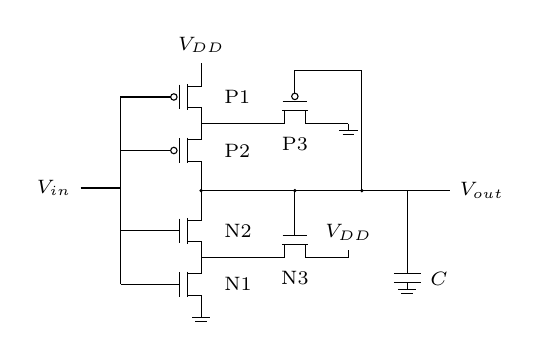
\begin{tikzpicture}[scale=0.68,font=\scriptsize]
\mos{1}{5}{}{1}\mos{1}{4}{}{1}\mos{1}{2.5}{}{0}\mos{1}{1.5}{}{0}
\rail{1.25}{5.5}{V_{DD}}\ground{1.25}{1}\draw(1.25,3)--(1.25,3.5);\draw(1.25,3.25)--(5.9,3.25)node[right]{$V_{out}$};\fill(1.25,3.25)circle(1pt);
\draw(-.25,1.5)--(-.25,5)--(.25,5);\draw(-.25,4)--(.25,4);\draw(-.25,2.5)--(.25,2.5);\draw(-.25,1.5)--(.25,1.5);\draw(-1,3.3)--(-.25,3.3)node[pos=0,left]{$V_{in}$};
\node[right]at(1.5,5){P1};\node[right]at(1.5,4){P2};\node[right]at(1.5,2.5){N2};\node[right]at(1.5,1.5){N1};
\hmos{3}{4.75}{P3}{1}\draw(1.25,4.5)--(2.5,4.5);\hmos{3}{2.25}{N3}{0}\draw(1.25,2)--(2.5,2);
\draw(3,3)--(3,3.25);\fill(3,3.25)circle(1pt);\draw(3,5.5)--(4.25,5.5)--(4.25,3.25);\fill(4.25,3.25)circle(1pt);
\draw(3.5,4.5)--(4,4.5);\ground{4}{4.5}\draw(3.5,2)--(4,2);\rail{4}{2}{V_{DD}}
\draw(5.1,3.25)--(5.1,1.7);\draw(4.85,1.7)--(5.35,1.7);\draw(4.85,1.53)--(5.35,1.53);\ground{5.1}{1.53}\node[right]at(5.35,1.6){$C$};
\end{tikzpicture}\quad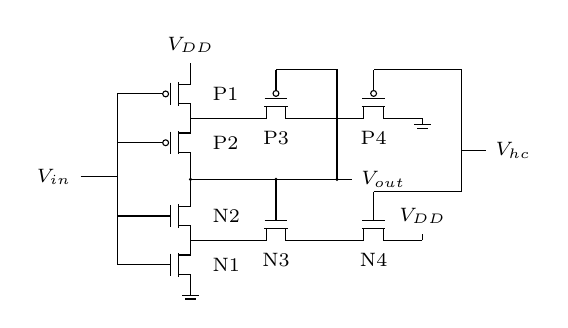
\begin{tikzpicture}[scale=0.62,font=\scriptsize]
\mos{1}{5}{}{1}\mos{1}{4}{}{1}\mos{1}{2.5}{}{0}\mos{1}{1.5}{}{0}
\rail{1.25}{5.5}{V_{DD}}\ground{1.25}{1}\draw(1.25,3)--(1.25,3.5);\draw(1.25,3.25)--(4.55,3.25)node[right]{$V_{out}$};\fill(1.25,3.25)circle(1pt);
\draw(-.25,1.5)--(-.25,5)--(.25,5);\draw(-.25,4)--(.25,4);\draw(-.25,2.5)--(.25,2.5);\draw(-.25,1.5)--(.25,1.5);\draw(-1,3.3)--(-.25,3.3)node[pos=0,left]{$V_{in}$};
\node[right]at(1.5,5){P1};\node[right]at(1.5,4){P2};\node[right]at(1.5,2.5){N2};\node[right]at(1.5,1.5){N1};
\hmos{3}{4.75}{P3}{1}\draw(1.25,4.5)--(2.5,4.5);\hmos{3}{2.25}{N3}{0}\draw(1.25,2)--(2.5,2);
\draw(3,3)--(3,3.25);\fill(3,3.25)circle(1pt);\draw(3,5.5)--(4.25,5.5)--(4.25,3.25);\fill(4.25,3.25)circle(1pt);
\hmos{5}{4.75}{P4}{1}\draw(3.5,4.5)--(4.5,4.5);\draw(5.5,4.5)--(6,4.5);\ground{6}{4.5}
\hmos{5}{2.25}{N4}{0}\draw(3.5,2)--(4.5,2);\draw(5.5,2)--(6,2);\rail{6}{2}{V_{DD}}
\draw(5,3)--(6.8,3)--(6.8,5.5)--(5,5.5);\draw(6.8,3.85)--(7.3,3.85)node[right]{$V_{hc}$};
\end{tikzpicture}\end{center}
Here $C$ is the explicitly drawn output load. It is not defined as N1's individual gate capacitance.
\newpage
\textbf{2(a), continued.}
Using the course fixed-resistance threshold model, the internal NMOS junction at the rising threshold is $u_n=V_T^+-V_{tn}=1.0$ V. The feedback path gives
\[u_n=\frac{R_{N1}}{R_{N1}+R_{N3}}V_{DD},\quad\text{so }R_{N3}=R_{N1}=R.\]
The upper PMOS junction at the falling threshold is $u_p=V_T^-+|V_{tp}|=1.0$ V, which gives $R_{P3}=R_{P1}$. The timing targets give
\[(R_{N1}+R_{N2})C=2RC\Rightarrow R_{N2}=R,\qquad R_{P1}+R_{P2}=2R.\]
One balanced valid choice is all six resistances equal to $R$. Since $\mu_n=2\mu_p$ and all lengths are 40 nm, this requires:
\begin{center}\begin{tabular}{lrr}\toprule Device & Width (nm) & Length (nm)\\\midrule N1 &100&40\\N2&100&40\\N3&100&40\\P1&200&40\\P2&200&40\\P3&200&40\\\bottomrule\end{tabular}\end{center}
It gives $V_T^+=1.0+0.4=1.4$ V, $V_T^-=1.0-0.4=0.6$ V and $t_r=t_f=2RC$ in the stated model.

The PMOS sizing is not unique without a balancing condition: with $0<a<2$, $R_{P1}=R_{P3}=aR$ and $R_{P2}=(2-a)R$ satisfy the same three constraints. Corresponding widths are $W_{P1}=W_{P3}=200/a$ nm and $W_{P2}=200/(2-a)$ nm. The balanced $a=1$ choice matches the student's valid final values and avoids inventing a uniqueness claim.

\textbf{(b)} P4 and N4 are \emph{in series} with the existing P3 and N3 feedback paths. N4 is controlled by $V_{hc}$. Increasing $V_{hc}$ strengthens N4, reducing its on-resistance and strengthening the feedback pull-up into $u_n$. In the conducting range,
\[u_n\simeq\frac{R_{N1}}{R_{N1}+R_{N3}+R_{N4}(V_{hc})}V_{DD},\qquad V_T^+\simeq u_n+V_{tn}.\]
Hence $R_{N4}\downarrow\Rightarrow u_n\uparrow\Rightarrow V_T^+\uparrow$:
\[\boxed{\text{Increase }V_{hc}\text{ to raise }V_T^+.}\]
P4 also changes the opposite feedback path, so this is not a claim that only the upper threshold changes. At cutoff or voltage limits, a constant-resistance formula needs replacement by actual MOS current equations. The later typed answer gives the correct direction; the series-path derivation supplies the reason.
\newpage
\textbf{3. Dynamic and differential split-level logic (10 points)}
The original has one full-expression complement: $f=\overline{AB(C+D)}$. Its complementary conduction condition is $h=AB(C+D)$; by De Morgan $f=\bar A+\bar B+\bar C\bar D$.

\textbf{Dynamic logic.} Precharge output $f$ to $V_{DD}$ with a PMOS gated by $\phi$, and evaluate with NMOS $A$--$B$--$(C\parallel D)$ plus a $\phi$ footer:
\begin{center}\begin{tikzpicture}[x=.8cm,y=.82cm,font=\scriptsize]
\mos{0}{0.0}{\phi}{1}\node[right]at(0.45,0.45){$\mathrm{Ppre}$};\node[above]at(0.25,0.5){$V_{DD}$};\node[below]at(0.25,-0.5){$f$};
\mos{5}{0.0}{A}{0}\node[right]at(5.45,0.45){$\mathrm{N_A}$};\node[above]at(5.25,0.5){$f$};\node[below]at(5.25,-0.5){$d1$};
\mos{10}{0.0}{B}{0}\node[right]at(10.45,0.45){$\mathrm{N_B}$};\node[above]at(10.25,0.5){$d1$};\node[below]at(10.25,-0.5){$d2$};
\mos{0}{-2.25}{C}{0}\node[right]at(0.45,-1.8){$\mathrm{N_C}$};\node[above]at(0.25,-1.75){$d2$};\node[below]at(0.25,-2.75){$d3$};
\mos{5}{-2.25}{D}{0}\node[right]at(5.45,-1.8){$\mathrm{N_D}$};\node[above]at(5.25,-1.75){$d2$};\node[below]at(5.25,-2.75){$d3$};
\mos{10}{-2.25}{\phi}{0}\node[right]at(10.45,-1.8){$\mathrm{Nclk}$};\node[above]at(10.25,-1.75){$d3$};\node[below]at(10.25,-2.75){$0$};
\end{tikzpicture}\end{center}
When $\phi=1$, output $f$ discharges exactly when $h=1$. No extra inverter is inserted, because that would make the output $h$ instead of the requested $f$. The 6-MOS dynamic circuit requires the standard evaluation protocol and retention limits.

\textbf{Differential split-level (DSL).} Use complementary NMOS networks below low-swing nodes $p,q$. The $p$ network implements $h$ and the $q$ network implements $f$. Each full-swing output $f,g$ connects to its low-swing node through an NMOS with gate $V_{ref}$. The PMOS load on $f$ is gated by \emph{opposite internal node} $q$, and the PMOS load on $g$ by $p$. The next page draws all 12 core transistors with these net labels.
\newpage
\textbf{3. DSL transistor schematic, continued.}
\begin{center}\begin{tikzpicture}[x=.8cm,y=.82cm,font=\scriptsize]
\mos{0}{0.0}{q}{1}\node[right]at(0.45,0.45){$\mathrm{P_f}$};\node[above]at(0.25,0.5){$V_{DD}$};\node[below]at(0.25,-0.5){$f$};
\mos{5}{0.0}{p}{1}\node[right]at(5.45,0.45){$\mathrm{P_g}$};\node[above]at(5.25,0.5){$V_{DD}$};\node[below]at(5.25,-0.5){$g$};
\mos{10}{0.0}{V_{ref}}{0}\node[right]at(10.45,0.45){$\mathrm{Nref_f}$};\node[above]at(10.25,0.5){$f$};\node[below]at(10.25,-0.5){$p$};
\mos{0}{-2.25}{V_{ref}}{0}\node[right]at(0.45,-1.8){$\mathrm{Nref_g}$};\node[above]at(0.25,-1.75){$g$};\node[below]at(0.25,-2.75){$q$};
\mos{5}{-2.25}{A}{0}\node[right]at(5.45,-1.8){$\mathrm{N_A}$};\node[above]at(5.25,-1.75){$p$};\node[below]at(5.25,-2.75){$p1$};
\mos{10}{-2.25}{B}{0}\node[right]at(10.45,-1.8){$\mathrm{N_B}$};\node[above]at(10.25,-1.75){$p1$};\node[below]at(10.25,-2.75){$p2$};
\mos{0}{-4.5}{C}{0}\node[right]at(0.45,-4.05){$\mathrm{N_C}$};\node[above]at(0.25,-4.0){$p2$};\node[below]at(0.25,-5.0){$0$};
\mos{5}{-4.5}{D}{0}\node[right]at(5.45,-4.05){$\mathrm{N_D}$};\node[above]at(5.25,-4.0){$p2$};\node[below]at(5.25,-5.0){$0$};
\mos{10}{-4.5}{\bar A}{0}\node[right]at(10.45,-4.05){$\mathrm{N_a}$};\node[above]at(10.25,-4.0){$q$};\node[below]at(10.25,-5.0){$0$};
\mos{0}{-6.75}{\bar B}{0}\node[right]at(0.45,-6.3){$\mathrm{N_b}$};\node[above]at(0.25,-6.25){$q$};\node[below]at(0.25,-7.25){$0$};
\mos{5}{-6.75}{\bar C}{0}\node[right]at(5.45,-6.3){$\mathrm{N_c}$};\node[above]at(5.25,-6.25){$q$};\node[below]at(5.25,-7.25){$q1$};
\mos{10}{-6.75}{\bar D}{0}\node[right]at(10.45,-6.3){$\mathrm{N_d}$};\node[above]at(10.25,-6.25){$q1$};\node[below]at(10.25,-7.25){$0$};
\end{tikzpicture}\end{center}
Repeated names denote connected electrical terminals. Here $g=\bar f=h$ is the complementary full-swing output. The opposite \emph{low-swing} load-control connections and the two $V_{ref}$ NMOS distinguish DSL from ordinary cross-coupled differential CMOS. Choose the reference so the low-swing internal high is roughly $V_{ref}-V_{tn}$ while the output can rise to $V_{DD}$; device currents and ratio choices must support the desired output levels. DSL can have static contention because its PMOS load gate does not rise fully to $V_{DD}$.

The complementary input generators add the following eight MOS (four ordinary static CMOS inverters):
\begin{center}\begin{tikzpicture}[x=.8cm,y=.82cm,font=\scriptsize]
\mos{0}{0.0}{A}{1}\node[right]at(0.45,0.45){$\mathrm{PgenA}$};\node[above]at(0.25,0.5){$V_{DD}$};\node[below]at(0.25,-0.5){$\bar A$};
\mos{5}{0.0}{A}{0}\node[right]at(5.45,0.45){$\mathrm{NgenA}$};\node[above]at(5.25,0.5){$\bar A$};\node[below]at(5.25,-0.5){$0$};
\mos{10}{0.0}{B}{1}\node[right]at(10.45,0.45){$\mathrm{PgenB}$};\node[above]at(10.25,0.5){$V_{DD}$};\node[below]at(10.25,-0.5){$\bar B$};
\mos{0}{-2.25}{B}{0}\node[right]at(0.45,-1.8){$\mathrm{NgenB}$};\node[above]at(0.25,-1.75){$\bar B$};\node[below]at(0.25,-2.75){$0$};
\mos{5}{-2.25}{C}{1}\node[right]at(5.45,-1.8){$\mathrm{PgenC}$};\node[above]at(5.25,-1.75){$V_{DD}$};\node[below]at(5.25,-2.75){$\bar C$};
\mos{10}{-2.25}{C}{0}\node[right]at(10.45,-1.8){$\mathrm{NgenC}$};\node[above]at(10.25,-1.75){$\bar C$};\node[below]at(10.25,-2.75){$0$};
\mos{0}{-4.5}{D}{1}\node[right]at(0.45,-4.05){$\mathrm{PgenD}$};\node[above]at(0.25,-4.0){$V_{DD}$};\node[below]at(0.25,-5.0){$\bar D$};
\mos{5}{-4.5}{D}{0}\node[right]at(5.45,-4.05){$\mathrm{NgenD}$};\node[above]at(5.25,-4.0){$\bar D$};\node[below]at(5.25,-5.0){$0$};
\end{tikzpicture}\end{center}
The core count is 12; with these generators it is 20. The student's DSL sketch has the correct reference-clamp idea, which is retained after checking against the lecturer's Chapter 6, slide 32.
\textbf{Primary reference:} \url{https://www.ee.ncu.edu.tw/jfli/public_html/VLSI/lecture/ch06.pdf}, slides 32--33 (DSL) and 13--18 (dynamic limitations). No reference-voltage numeric value is specified by the question.
\newpage
\textbf{4. Symbolic layout extraction (10 points)}
\begin{center}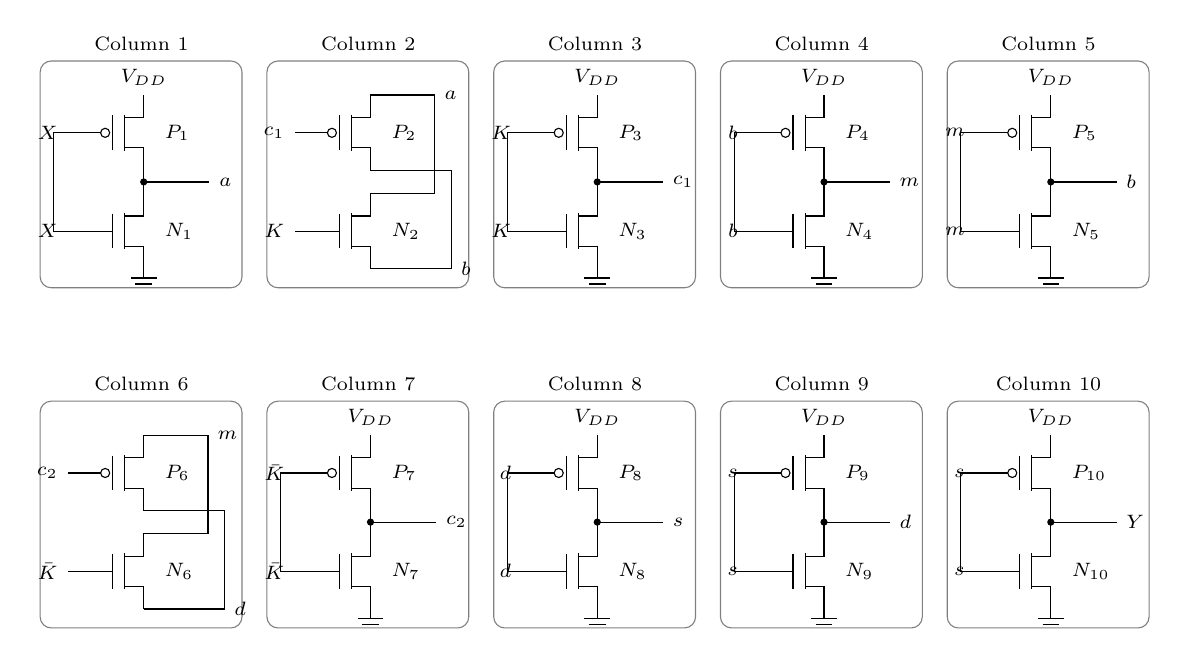
\begin{tikzpicture}[x=.96cm,y=.96cm,font=\small]
\begin{scope}[shift={(0.0,3.7)}]
\draw[gray,rounded corners](-1.12,-1.4)rectangle(1.55,1.6);
\node[font=\scriptsize]at(.22,1.83){Column 1};
\mos{0}{.65}{X}{1}
\mos{0}{-.65}{X}{0}
\node[right,font=\scriptsize]at(.4,.65){$P_{1}$};
\node[right,font=\scriptsize]at(.4,-.65){$N_{1}$};
\draw(.25,.15)--(.25,-.15);
\node[above,font=\scriptsize]at(.25,1.15){$V_{DD}$};
\gnd{.25}{-1.15}
\draw(.25,0)--(1.12,0)node[right,font=\scriptsize]{$a$};
\fill(.25,0)circle(1.3pt);
\draw(-.75,.65)--(-.94,.65)--(-.94,-.65)--(-.75,-.65);
\end{scope}
\begin{scope}[shift={(3.0,3.7)}]
\draw[gray,rounded corners](-1.12,-1.4)rectangle(1.55,1.6);
\node[font=\scriptsize]at(.22,1.83){Column 2};
\mos{0}{.65}{c_1}{1}
\mos{0}{-.65}{K}{0}
\node[right,font=\scriptsize]at(.4,.65){$P_{2}$};
\node[right,font=\scriptsize]at(.4,-.65){$N_{2}$};
\draw(.25,1.15)--(1.1,1.15)--(1.1,-.15)--(.25,-.15);
\draw(.25,.15)--(1.32,.15)--(1.32,-1.15)--(.25,-1.15);
\node[right,font=\scriptsize]at(1.1,1.15){$a$};
\node[right,font=\scriptsize]at(1.32,-1.15){$b$};
\end{scope}
\begin{scope}[shift={(6.0,3.7)}]
\draw[gray,rounded corners](-1.12,-1.4)rectangle(1.55,1.6);
\node[font=\scriptsize]at(.22,1.83){Column 3};
\mos{0}{.65}{K}{1}
\mos{0}{-.65}{K}{0}
\node[right,font=\scriptsize]at(.4,.65){$P_{3}$};
\node[right,font=\scriptsize]at(.4,-.65){$N_{3}$};
\draw(.25,.15)--(.25,-.15);
\node[above,font=\scriptsize]at(.25,1.15){$V_{DD}$};
\gnd{.25}{-1.15}
\draw(.25,0)--(1.12,0)node[right,font=\scriptsize]{$c_1$};
\fill(.25,0)circle(1.3pt);
\draw(-.75,.65)--(-.94,.65)--(-.94,-.65)--(-.75,-.65);
\end{scope}
\begin{scope}[shift={(9.0,3.7)}]
\draw[gray,rounded corners](-1.12,-1.4)rectangle(1.55,1.6);
\node[font=\scriptsize]at(.22,1.83){Column 4};
\mos{0}{.65}{b}{1}
\mos{0}{-.65}{b}{0}
\node[right,font=\scriptsize]at(.4,.65){$P_{4}$};
\node[right,font=\scriptsize]at(.4,-.65){$N_{4}$};
\draw(.25,.15)--(.25,-.15);
\node[above,font=\scriptsize]at(.25,1.15){$V_{DD}$};
\gnd{.25}{-1.15}
\draw(.25,0)--(1.12,0)node[right,font=\scriptsize]{$m$};
\fill(.25,0)circle(1.3pt);
\draw(-.75,.65)--(-.94,.65)--(-.94,-.65)--(-.75,-.65);
\end{scope}
\begin{scope}[shift={(12.0,3.7)}]
\draw[gray,rounded corners](-1.12,-1.4)rectangle(1.55,1.6);
\node[font=\scriptsize]at(.22,1.83){Column 5};
\mos{0}{.65}{m}{1}
\mos{0}{-.65}{m}{0}
\node[right,font=\scriptsize]at(.4,.65){$P_{5}$};
\node[right,font=\scriptsize]at(.4,-.65){$N_{5}$};
\draw(.25,.15)--(.25,-.15);
\node[above,font=\scriptsize]at(.25,1.15){$V_{DD}$};
\gnd{.25}{-1.15}
\draw(.25,0)--(1.12,0)node[right,font=\scriptsize]{$b$};
\fill(.25,0)circle(1.3pt);
\draw(-.75,.65)--(-.94,.65)--(-.94,-.65)--(-.75,-.65);
\end{scope}
\begin{scope}[shift={(0.0,-0.8)}]
\draw[gray,rounded corners](-1.12,-1.4)rectangle(1.55,1.6);
\node[font=\scriptsize]at(.22,1.83){Column 6};
\mos{0}{.65}{c_2}{1}
\mos{0}{-.65}{\bar K}{0}
\node[right,font=\scriptsize]at(.4,.65){$P_{6}$};
\node[right,font=\scriptsize]at(.4,-.65){$N_{6}$};
\draw(.25,1.15)--(1.1,1.15)--(1.1,-.15)--(.25,-.15);
\draw(.25,.15)--(1.32,.15)--(1.32,-1.15)--(.25,-1.15);
\node[right,font=\scriptsize]at(1.1,1.15){$m$};
\node[right,font=\scriptsize]at(1.32,-1.15){$d$};
\end{scope}
\begin{scope}[shift={(3.0,-0.8)}]
\draw[gray,rounded corners](-1.12,-1.4)rectangle(1.55,1.6);
\node[font=\scriptsize]at(.22,1.83){Column 7};
\mos{0}{.65}{\bar K}{1}
\mos{0}{-.65}{\bar K}{0}
\node[right,font=\scriptsize]at(.4,.65){$P_{7}$};
\node[right,font=\scriptsize]at(.4,-.65){$N_{7}$};
\draw(.25,.15)--(.25,-.15);
\node[above,font=\scriptsize]at(.25,1.15){$V_{DD}$};
\gnd{.25}{-1.15}
\draw(.25,0)--(1.12,0)node[right,font=\scriptsize]{$c_2$};
\fill(.25,0)circle(1.3pt);
\draw(-.75,.65)--(-.94,.65)--(-.94,-.65)--(-.75,-.65);
\end{scope}
\begin{scope}[shift={(6.0,-0.8)}]
\draw[gray,rounded corners](-1.12,-1.4)rectangle(1.55,1.6);
\node[font=\scriptsize]at(.22,1.83){Column 8};
\mos{0}{.65}{d}{1}
\mos{0}{-.65}{d}{0}
\node[right,font=\scriptsize]at(.4,.65){$P_{8}$};
\node[right,font=\scriptsize]at(.4,-.65){$N_{8}$};
\draw(.25,.15)--(.25,-.15);
\node[above,font=\scriptsize]at(.25,1.15){$V_{DD}$};
\gnd{.25}{-1.15}
\draw(.25,0)--(1.12,0)node[right,font=\scriptsize]{$s$};
\fill(.25,0)circle(1.3pt);
\draw(-.75,.65)--(-.94,.65)--(-.94,-.65)--(-.75,-.65);
\end{scope}
\begin{scope}[shift={(9.0,-0.8)}]
\draw[gray,rounded corners](-1.12,-1.4)rectangle(1.55,1.6);
\node[font=\scriptsize]at(.22,1.83){Column 9};
\mos{0}{.65}{s}{1}
\mos{0}{-.65}{s}{0}
\node[right,font=\scriptsize]at(.4,.65){$P_{9}$};
\node[right,font=\scriptsize]at(.4,-.65){$N_{9}$};
\draw(.25,.15)--(.25,-.15);
\node[above,font=\scriptsize]at(.25,1.15){$V_{DD}$};
\gnd{.25}{-1.15}
\draw(.25,0)--(1.12,0)node[right,font=\scriptsize]{$d$};
\fill(.25,0)circle(1.3pt);
\draw(-.75,.65)--(-.94,.65)--(-.94,-.65)--(-.75,-.65);
\end{scope}
\begin{scope}[shift={(12.0,-0.8)}]
\draw[gray,rounded corners](-1.12,-1.4)rectangle(1.55,1.6);
\node[font=\scriptsize]at(.22,1.83){Column 10};
\mos{0}{.65}{s}{1}
\mos{0}{-.65}{s}{0}
\node[right,font=\scriptsize]at(.4,.65){$P_{10}$};
\node[right,font=\scriptsize]at(.4,-.65){$N_{10}$};
\draw(.25,.15)--(.25,-.15);
\node[above,font=\scriptsize]at(.25,1.15){$V_{DD}$};
\gnd{.25}{-1.15}
\draw(.25,0)--(1.12,0)node[right,font=\scriptsize]{$Y$};
\fill(.25,0)circle(1.3pt);
\draw(-.75,.65)--(-.94,.65)--(-.94,-.65)--(-.75,-.65);
\end{scope}
\end{tikzpicture}\\All 20 MOS devices. Repeated net names denote electrical connections; column numbers follow the original left to right.\end{center}

In the column diagram, the short labels $K=CLK$ and $\bar K=CLKB$ denote the same externally supplied clock pair; net labels $a,b,c_1,c_2,d,m,s$ are analysis names.
The original contains \textbf{20 MOS: 10 PMOS and 10 NMOS}, grouped as eight inverters and two transmission gates. From left to right, the contact-extracted structure is
\[X\xrightarrow{INV}a\overset{TG_M}{\longleftrightarrow}b\xrightarrow{INV}m\overset{TG_S}{\longleftrightarrow}d\xrightarrow{INV}s\xrightarrow{INV}Y.\]
The master feedback inverter connects $m\to b$, and the slave feedback inverter connects $s\to d$ continuously. The local clock inverters generate $c_1=\overline{CLK}$ and $c_2=\overline{CLKB}$, where the externally labeled $CLKB=\overline{CLK}$. Master TG gates are $p:c_1,n:CLK$; slave TG gates are $p:c_2,n:CLKB$. Thus the master input is enabled at $CLK=1$ and the slave input at $CLK=0$.

With successful writes, the two-stage latch arrangement conditionally stores $Y=X$ on the falling clock edge. This behavior requires the enabled upstream driver/TG to override the \emph{always-connected} feedback inverter. The original gives no drive strengths or dimensions, so write margin is not proved, and the feedback devices are not relabeled ``weak.'' The extraction is retained exactly; no second feedback TG is invented to turn it into a different latch. In the ideal graph checks, 8 settled states are rail-consistent and 8 attempted opposite writes expose contention, which is an expected ratioed-latch limitation rather than a verification omission.

This circuit family matches the continuously connected feedback latch in the lecturer's Chapter 7, slide 9 (upper schematic); the two-TG latch shown on slide 10 is not an exact contact match. Primary reference: \url{https://www.ee.ncu.edu.tw/jfli/public_html/VLSI/lecture/ch07.pdf}.
\textbf{Extraction notes.} See \texttt{layout-connectivity.json} for the column-by-column net table and clock phases, and \texttt{layout-checks.csv} for the ideal switch verification. Only drawn black contacts join layers. A metal/poly crossing without a contact remains insulated; adjacent diffusion regions separated by a gate form a MOS rather than one shorted wire. The student sketch received no Q4 credit and the later notes admit it was improvised; it is not used as the transistor graph authority.
\newpage
\textbf{5. Super buffer and switching (20 points)}
\textbf{(a)} The electrical effort is $H=C_L/C_g=2.98\mathrm{pF}/1\mathrm{fF}=2980\simeq e^8$. For a chain with first input load $C_g$, no parasitic delay, and proportional sizing, equal stage efforts minimize the sum of RC delays. A chain of $N$ inverters gives $T_N=N H^{1/N}\tau$, where $\tau=R_{inv,min}C_g$ is the stipulated resistance-model unit. Continuous minimization gives $N=\ln H\simeq8$. Choose \emph{eight} inverters, also preserving the input/output polarity.

Let $r=H^{1/8}\simeq2.71817$. Stage $i=1,\ldots,8$ has $C_{in,i}=r^{i-1}C_g$, with each NMOS/PMOS width $r^{i-1}W_{min}$ and length $L_{min}$:
\begin{center}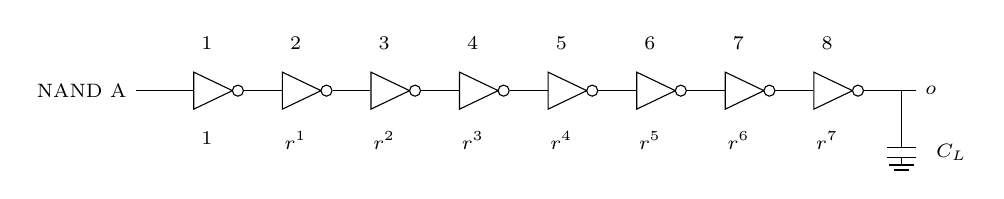
\begin{tikzpicture}[x=.9cm,y=.8cm,font=\scriptsize]
\node[not gate US,draw,minimum width=.55cm](b0)at(0.0,0){};\node[above]at(0.0,.5){1};\node[below]at(0.0,-.5){$1$};
\node[not gate US,draw,minimum width=.55cm](b1)at(1.25,0){};\node[above]at(1.25,.5){2};\node[below]at(1.25,-.5){$r^1$};
\draw(b0.output)--(b1.input);
\node[not gate US,draw,minimum width=.55cm](b2)at(2.5,0){};\node[above]at(2.5,.5){3};\node[below]at(2.5,-.5){$r^2$};
\draw(b1.output)--(b2.input);
\node[not gate US,draw,minimum width=.55cm](b3)at(3.75,0){};\node[above]at(3.75,.5){4};\node[below]at(3.75,-.5){$r^3$};
\draw(b2.output)--(b3.input);
\node[not gate US,draw,minimum width=.55cm](b4)at(5.0,0){};\node[above]at(5.0,.5){5};\node[below]at(5.0,-.5){$r^4$};
\draw(b3.output)--(b4.input);
\node[not gate US,draw,minimum width=.55cm](b5)at(6.25,0){};\node[above]at(6.25,.5){6};\node[below]at(6.25,-.5){$r^5$};
\draw(b4.output)--(b5.input);
\node[not gate US,draw,minimum width=.55cm](b6)at(7.5,0){};\node[above]at(7.5,.5){7};\node[below]at(7.5,-.5){$r^6$};
\draw(b5.output)--(b6.input);
\node[not gate US,draw,minimum width=.55cm](b7)at(8.75,0){};\node[above]at(8.75,.5){8};\node[below]at(8.75,-.5){$r^7$};
\draw(b6.output)--(b7.input);
\draw(b0.input)--(-1,0)node[left]{NAND A};\draw(b7.output)--(10,0)node[right]{$o$};\draw(9.8,0)--(9.8,-.9);\draw(9.6,-.9)--(10,-.9);\draw(9.6,-1.06)--(10,-1.06);\ground{9.8}{-1.06}\node[right]at(10.15,-.98){$C_L$};
\end{tikzpicture}\end{center}
\begin{center}\begin{tabular}{crr}\toprule Stage & $C_{in}/C_g$ & Each width / $W_{min}$\\\midrule 1&1&1\\2&2.7182&2.7182\\3&7.3885&7.3885\\4&20.0831&20.0831\\5&54.5894&54.5894\\6&148.383&148.383\\7&403.332&403.332\\8&1096.33&1096.33\\\bottomrule\end{tabular}\end{center}
The last stage sees $C_L=r^8 C_g=2980C_g$, so every effort equals $r$. The delay is $T_{min}\simeq8r\tau=21.745\tau$. Using the question's rounded $e$ values is acceptable, but every inverter size must be stated. The student's eight-stage concept is retained and the missing size labels are made explicit.

\textbf{(b)(i)} The settled functions are $u=\bar x$, $v=x$, $w=\overline{uy}=x+\bar y$, and $o=\overline{vw}=\bar x$. Their cycle is
\begin{center}\begin{tabular}{cccccc}\toprule $xy$ & $u$ & $v$ & $w$ & $o$ & Next step\\\midrule 00&1&0&1&1&01\\01&1&0&0&1&10\\10&0&1&1&0&11\\11&0&1&1&0&00\\\bottomrule\end{tabular}\end{center}
Every node has two total transitions but only one $0\to1$ charging event in four steps. Thus $\alpha_{all}=2/4=0.5$ and $\alpha_{01}=1/4=0.25$. The student's later note ``0.5'' is valid for \emph{all transitions}; it must not be inserted into the charging-event power formula without its factor of one-half.
\newpage
\textbf{5(b)(ii). Dynamic power of the buffer.}
Define $f$ as the input-step frequency (one of the four transitions per $1/f$). A fully settled buffer output switches twice in the four-step sequence, so every stage has $\alpha_{01}=1/4$. Buffer output loads are $rC_g,r^2C_g,\ldots,r^7C_g,C_L=r^8C_g$. Hence
\[\boxed{P_{buffer}=\frac14 fV_{dd}^2 C_g\sum_{i=1}^{8}r^i
=\frac14fV_{dd}^2 C_g\frac{r(r^8-1)}{r-1}.}\]
With $C_g=1$ fF, $\sum C=4.71282$ pF, giving $P_{buffer}\simeq1.17820\times10^{-12}fV_{dd}^2$ W when $f$ is in Hz and $V_{dd}$ in volts.
The first inverter's input capacitance $C_g$ is driven by NAND A, so its charging loss is attributed to the NAND driver rather than counted as an extra buffer output load. If total circuit power is requested, that upstream $C_g$ term and all other upstream loads must be included separately. Equivalently, $P=(1/2)\alpha_{all} f V_{dd}^2\sum C$ with $\alpha_{all}=0.5$. If $f$ instead denotes whole four-step cycles per second, use $f_{step}=4f$ and one charging event per cycle. No numerical $V_{dd}$ or frequency is supplied.

\textbf{5(b)(iii). Glitch scope.} For ideal simultaneous input steps in the stated sequence, and enough time for each state to settle, there are no additional transitions in $u,v,w,o$. In $00\to01$, the $w$ falling transition is masked by $v=0$; in $01\to10$, $u$ and $y$ both fall and $w$ rises while $v$ rises, so $o$ falls only once. In $10\to11$, $u=0$ masks the $y$ rise. In $11\to00$, $y$ falls immediately before the delayed $u$ rise, keeping $w=1$ while $v$ falls, so $o$ rises only once.

Equal NAND delays by themselves do \emph{not} guarantee a glitch-free physical circuit: input skew and the two inverter delays still matter. For a concrete allowed-delay example, let both inverters delay 1 unit and both NANDs delay 0.1 unit. On $11\to00$, let $x$ fall at time 0 and $y$ fall at time 1.5. Then $u$ rises at 1, $w$ falls at 1.1, and $o$ rises at 1.2; after $y$ falls, $w$ rises at 1.6 and $o$ falls at 1.7; when $v$ falls at 2, $o$ rises at 2.1. The extra pulse exists despite matched NAND delays.

Accordingly, the ideal-cycle activity above is the settled, unskewed result, and extra glitch energy under other timing assumptions must be added if those assumptions are supplied. The student's broad glitch warning is retained with a correct scope and a constructive example, rather than claiming it must occur in every listed ideal step.
\newpage
\textbf{6. Incomplete timing question -- cannot answer and skipped}
The supplied original loses numerical timing premises and Q6(a),(b). Q6(c) and Fig. 5 remain readable, but ``twice the original frequency'' cannot be evaluated or verified without the original period/path parameters. No register insertion solution, no copied 2 ns/1 GHz values, and no guessed timing assumptions are provided. A pipeline must also balance cycle latency on reconvergent operands; the student's added registers are expressly noted as functionally wrong in the later answer note.
\begin{center}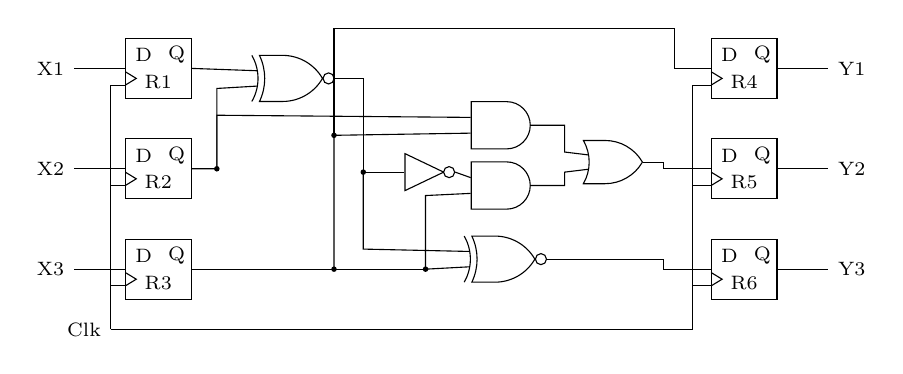
\begin{tikzpicture}[x=.93cm,y=.85cm,font=\scriptsize]
\foreach\r/\y in {1/4,2/2.5,3/1}{\draw(0,\y-.45)rectangle(.9,\y+.45);\node at(.25,\y+.2){D};\node at(.7,\y+.2){Q};\node at(.45,\y-.2){R\r};\draw(-.7,\y)--(0,\y);\node[left]at(-.7,\y){X\r};\draw(0,\y-.25)--(.15,\y-.15)--(0,\y-.05);}
\foreach\r/\y/\o in {4/4/Y1,5/2.5/Y2,6/1/Y3}{\draw(8,\y-.45)rectangle(8.9,\y+.45);\node at(8.25,\y+.2){D};\node at(8.7,\y+.2){Q};\node at(8.45,\y-.2){R\r};\draw(8.9,\y)--(9.6,\y)node[right]{\o};\draw(8,\y-.25)--(8.15,\y-.15)--(8,\y-.05);}
\draw(-.2,.1)node[left]{Clk}--(7.75,.1);\draw(-.2,.1)--(-.2,3.75);\foreach\y in {3.75,2.25,.75}{\draw(-.2,\y)--(0,\y);}\draw(7.75,.1)--(7.75,3.75);\foreach\y in {3.75,2.25,.75}{\draw(7.75,\y)--(8,\y);}
\node[xnor gate US,draw,logic gate inputs=nn,minimum width=.8cm](s)at(2.2,3.85){};\draw(.9,4)--(s.input 1);\draw(.9,2.5)--(1.25,2.5)--(1.25,3.7)--(s.input 2);
\node[and gate US,draw,logic gate inputs=nn,minimum width=.75cm](h)at(5.1,3.15){};\node[and gate US,draw,logic gate inputs=nn,minimum width=.75cm](l)at(5.1,2.25){};\node[or gate US,draw,logic gate inputs=nn,minimum width=.75cm](o)at(6.6,2.6){};\node[not gate US,draw,minimum width=.55cm](n)at(4,2.45){};\node[xnor gate US,draw,logic gate inputs=nn,minimum width=.8cm](p)at(5.1,1.15){};
\draw(s.output)--(3.25,3.85)--(3.25,2.45)--(n.input);\draw(3.25,2.45)--(3.25,1.3)--(p.input 1);\fill(3.25,2.45)circle(1pt);
\draw(n.output)--(l.input 1);\draw(1.25,2.5)--(1.25,3.3)--(h.input 1);\fill(1.25,2.5)circle(1pt);
\draw(.9,1)--(4.1,1);\draw(2.85,1)--(2.85,3)--(h.input 2);\draw(2.85,3)--(2.85,4.6)--(7.5,4.6)--(7.5,4)--(8,4);\fill(2.85,3)circle(1pt);\fill(2.85,1)circle(1pt);\draw(4.1,1)--(p.input 2);\draw(4.1,1)--(4.1,2.1)--(l.input 2);\fill(4.1,1)circle(1pt);
\draw(h.output)--(6,3.15)--(6,2.75)--(o.input 1);\draw(l.output)--(6,2.25)--(6,2.45)--(o.input 2);\draw(o.output)--(7.35,2.6)--(7.35,2.5)--(8,2.5);\draw(p.output)--(7.35,1.15)--(7.35,1)--(8,1);
\end{tikzpicture}\end{center}
The retained diagram is editable; preserving a drawing does not restore missing timing conditions.

\textbf{7. Readable original short answers (a)--(c)}
\begin{enumerate}[label=(\alph*),leftmargin=7mm,itemsep=8pt]
\item Standard cells require a common row height (or a supported integer-height family) and aligned VDD/VSS rail heights/locations for legal abutment. Merely saying ``obey design rules'' is not the requested pair of standard-cell-library interface requirements. The student's rail-alignment idea is retained and the common-height requirement supplied.
\item Charge sharing/leakage can corrupt an unrefreshed dynamic node; simple single-phase NMOS dynamic stages cannot be directly cascaded because a precharged-high upstream output can incorrectly discharge a downstream node before evaluation settles. Domino adds a restoring inverter and requires monotonic evaluation inputs. The lecturer's Chapter 6, slide 13 lists charge sharing and direct-cascade limitations as the two course answers.
\item Design rules constrain physical geometry (widths, spacing, overlaps, enclosures and related process limits) so circuits can be manufactured reliably with adequate yield across process variation. They are process-dependent geometric requirements, not a truth-table design rule or a guarantee of zero analog variation.
\end{enumerate}
\newpage
\textbf{Separate unverified Q7 typed supplement}
The original Q7(d)--(f) wording and point labels are missing. The following are conditional conceptual notes for the retained secondary transcription, not restored original exam answers.
\begin{enumerate}[label=(\alph*),start=4,leftmargin=7mm,itemsep=9pt]
\item If the typed pseudo-NMOS question is accurate: its PMOS pull-up is continuously on. An active NMOS network must overpower it to produce an acceptable low level; $V_{OL}$ and noise margin depend on the pull-down/pull-up strength ratio. This is why pseudo-NMOS is ratioed, with DC contention when the output is low.
\item If the typed special-cell list is accurate: filler cells maintain row/well/rail continuity and satisfy abutment geometry; tap cells connect wells/substrate to their supply references and help control latch-up; endcap cells terminate row/block boundary geometry legally; decap cells provide local supply-to-ground charge storage to reduce transient supply variation. Exact legal implementations depend on the library/process. Endcaps are not a generic device that forbids all metal from leaving a block.
\item If the typed manufacturing/time-to-market question is accurate: gate-array and sea-of-gates approaches start with prefabricated transistor arrays and customize later interconnect layers, shortening per-design manufacturing lead time. Sea-of-gates is the channelless gate-array variant. This pair is supported by the lecturer's Chapter 5, slides 28--31, rather than justified only by the student's speculative note.
\end{enumerate}
\begin{flushleft}Primary references: \url{https://www.ee.ncu.edu.tw/jfli/public_html/VLSI/lecture/ch05.pdf} (standard cells, physical rules, gate arrays), \url{https://www.ee.ncu.edu.tw/jfli/public_html/VLSI/lecture/ch06.pdf} (dynamic limitations, DSL), and the primary references recorded in \texttt{SOURCES.md} for special cells.\end{flushleft}

\textbf{Verification.} \texttt{verify.py} checks dynamic truth/phase behavior, both DSL conduction networks, the Schmitt threshold/resistance/size equations, the optimized 8-stage taper, the four-state switching counts, ideal event traces, and the illustrative skew glitch. \texttt{layout-checks.csv} separately records contact-extracted latch behavior. These are ideal logic/connectivity and analytical checks, not HSPICE measurements or exact DSL analog load simulation.

Printed whole-question point labels sum to 105 and are preserved; complete answerable original parts cover Q1--Q5 plus Q7(a)--(c), while missing Q6 and original Q7(d)--(f) are explicitly skipped. Archive year attribution is 2021; the photographed paper has no printed year.
\end{document}
